\documentclass[tikz,border=12pt]{standalone}
\usepackage[utf8]{inputenc}
\usepackage[T1]{fontenc}
\usepackage{lmodern}
\usepackage{array}
\usepackage{tikz}
\usetikzlibrary{arrows.meta,calc}
\definecolor{greenFill}{HTML}{E8F5E9}
\definecolor{greenStroke}{HTML}{43A047}
\definecolor{coreFill}{HTML}{E1F5FE}
\definecolor{coreStroke}{HTML}{0277BD}
\newcommand{\classcontent}[2]{\begin{tabular}{p{5.8cm}}\centering\bfseries #1\tabularnewline\hline\raggedright\arraybackslash #2\end{tabular}}
\begin{document}
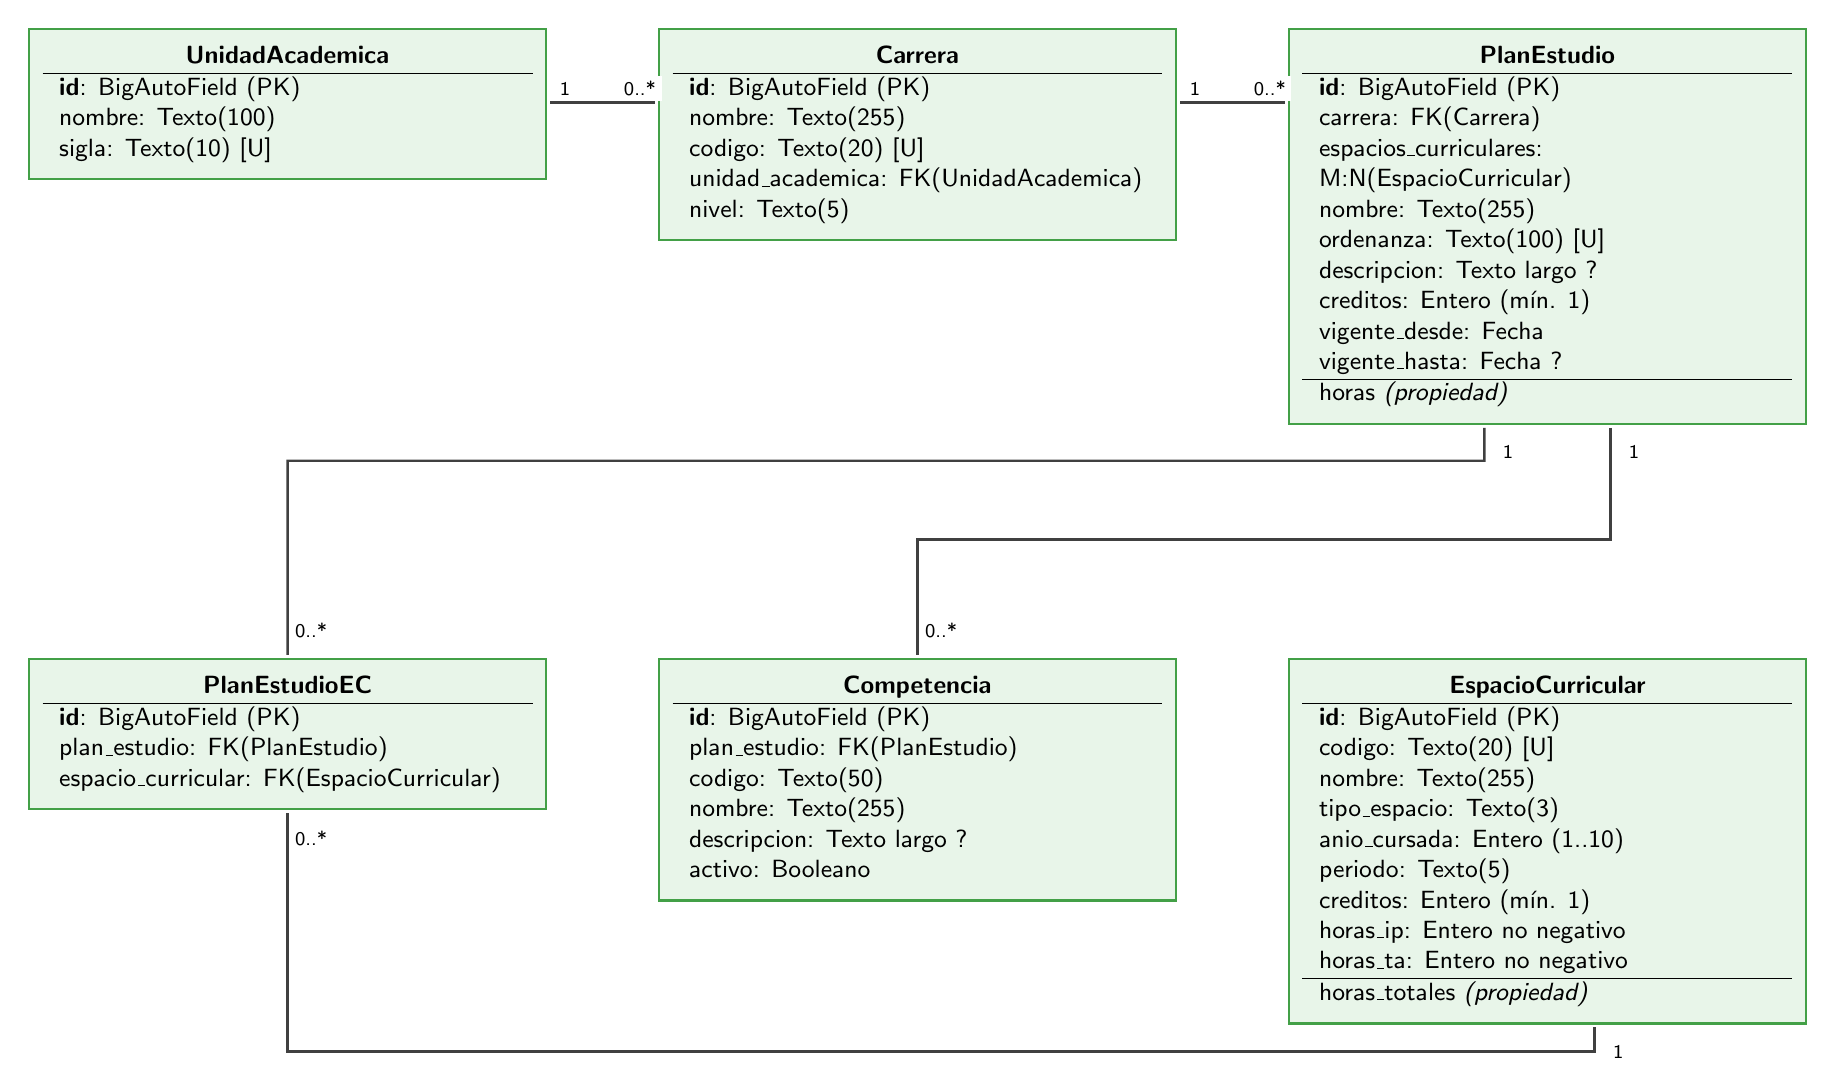
\begin{tikzpicture}[
 font=\sffamily\small,
 cls/.style={rectangle,draw=greenStroke,fill=greenFill,line width=.8pt,inner sep=5pt,anchor=north},
 ref/.style={cls,draw=coreStroke,fill=coreFill},
 association/.style={line width=.9pt,draw=black!75,shorten >=1pt,shorten <=1pt},
 dependency/.style={association,dashed,-{Stealth[length=3mm,width=2.2mm]}},
 mult/.style={font=\sffamily\scriptsize,fill=white,inner sep=2pt,text=black}
]
\node[cls] (UnidadAcademica) at (0,0) {\classcontent{UnidadAcademica}{\textbf{id}: BigAutoField (PK)\\nombre: Texto(100)\\sigla: Texto(10) [U]}};
\node[cls] (Carrera) at (8,0) {\classcontent{Carrera}{\textbf{id}: BigAutoField (PK)\\nombre: Texto(255)\\codigo: Texto(20) [U]\\unidad\_academica: FK(UnidadAcademica)\\nivel: Texto(5)}};
\node[cls] (PlanEstudio) at (16,0) {\classcontent{PlanEstudio}{\textbf{id}: BigAutoField (PK)\\carrera: FK(Carrera)\\espacios\_curriculares: M:N(EspacioCurricular)\\nombre: Texto(255)\\ordenanza: Texto(100) [U]\\descripcion: Texto largo ?\\creditos: Entero (mín. 1)\\vigente\_desde: Fecha\\vigente\_hasta: Fecha ?\\\hline horas \textit{(propiedad)}}};
\node[cls] (Competencia) at (8,-8) {\classcontent{Competencia}{\textbf{id}: BigAutoField (PK)\\plan\_estudio: FK(PlanEstudio)\\codigo: Texto(50)\\nombre: Texto(255)\\descripcion: Texto largo ?\\activo: Booleano}};
\node[cls] (PlanEstudioEC) at (0,-8) {\classcontent{PlanEstudioEC}{\textbf{id}: BigAutoField (PK)\\plan\_estudio: FK(PlanEstudio)\\espacio\_curricular: FK(EspacioCurricular)}};
\node[cls] (EspacioCurricular) at (16,-8) {\classcontent{EspacioCurricular}{\textbf{id}: BigAutoField (PK)\\codigo: Texto(20) [U]\\nombre: Texto(255)\\tipo\_espacio: Texto(3)\\anio\_cursada: Entero (1..10)\\periodo: Texto(5)\\creditos: Entero (mín. 1)\\horas\_ip: Entero no negativo\\horas\_ta: Entero no negativo\\\hline horas\_totales \textit{(propiedad)}}};
\draw[association] ($(UnidadAcademica.north east)+(0,-.95)$) -- ($(Carrera.north west)+(0,-.95)$) node[pos=.16,above,mult]{1} node[pos=.84,above,mult]{0..*};
\draw[association] ($(Carrera.north east)+(0,-.95)$) -- ($(PlanEstudio.north west)+(0,-.95)$) node[pos=.16,above,mult]{1} node[pos=.84,above,mult]{0..*};
\draw[association] ($(PlanEstudio.south)+(-.8,0)$) -- (15.2,-5.5) -- (0,-5.5) -- (PlanEstudioEC.north);
\node[mult] at ($(PlanEstudio.south)+(-.5,-.35)$) {1};
\node[mult] at ($(PlanEstudioEC.north)+(.3,.35)$) {0..*};
\draw[association] ($(PlanEstudio.south)+(.8,0)$) -- (16.8,-6.5) -- (8,-6.5) -- (Competencia.north);
\node[mult] at ($(PlanEstudio.south)+(1.1,-.35)$) {1};
\node[mult] at ($(Competencia.north)+(.3,.35)$) {0..*};
\draw[association] ($(EspacioCurricular.south)+(.6,0)$) -- (16.6,-13) -- (0,-13) -- (PlanEstudioEC.south);
\node[mult] at ($(EspacioCurricular.south)+(.9,-.35)$) {1};
\node[mult] at ($(PlanEstudioEC.south)+(.3,-.35)$) {0..*};
\end{tikzpicture}
\end{document}
